
%\documentclass[a4paper]{jarticle}


\section{msankey.rb sankeyダイアグラムの描画\label{sect:msankey}}
\index{msankey@msankey}
Sankeyダイアグラムとは,閉路のない有向グラフ(DAG:Directed Acyclic Graph)を視覚化する手法の一つで,
枝の重みとして定義される流量が接点間でどのような割合で流れていくかを直感的に理解することができ,
送電ネットワークの視覚化などに利用される.

内部では、D3ライブラリ(Data-Driven Documents)で作成された視覚化アプリケーションsankey diagram
(\url{http://bost.ocks.org/mike/sankey/})を利用している。

入力データとしては,表\ref{tbl:sankey_input1}に示されるような枝を節点ペアとその値を一行で示したCSVデータである。

出力はsankeyダイアグラムを組み込んだ単体のhtmlファイルで、
インターネットへの接続がなくてもブラウザがあれば描画できる(\ref{fig:sankey1})。
グラフの向きは左から右の方向で、コマンドパラメータ\verb|f=|で指定した1番目の項目が左、2番目の項目が右に対応する。
色のついたバーが節点に対応し、接点間を結ぶ帯が枝に対応する。
節点の出力位置の決定にはinterval relaxztion法が用いられている。
詳細はオリジナルのURL(上述)を参照のこと。
経験的には5節点$\times$水平位置10箇所$=50$節点ともなると、描画に非常に時間を要する。

なお、本コマンドを利用するためには、nysol/mcmdライブラリの他にjsonライブラリが必要となる。

\begin{table}[htbp]
\begin{center}
\begin{tabular}{c}

\begin{minipage}{0.12\hsize}
\begin{center}
\caption{入力データ(閉路のない有向グラフ)\label{tbl:sankey_input1}}
{\small
\begin{tabular}{cccc}
\hline
node1&node2&val\\
\hline
a&b&1\\
a&c&2\\
a&d&1\\
b&c&3\\
b&d&3\\
c&f&1\\
c&e&4\\
d&e&1\\
e&f&3\\
\hline
\end{tabular} 
}
\end{center}
\end{minipage}

\end{tabular} 
\end{center}
\end{table} 


\begin{figure}[htbp]
\begin{center}
\begin{tabular}{c}

\begin{minipage}{0.5\hsize}
\begin{center}
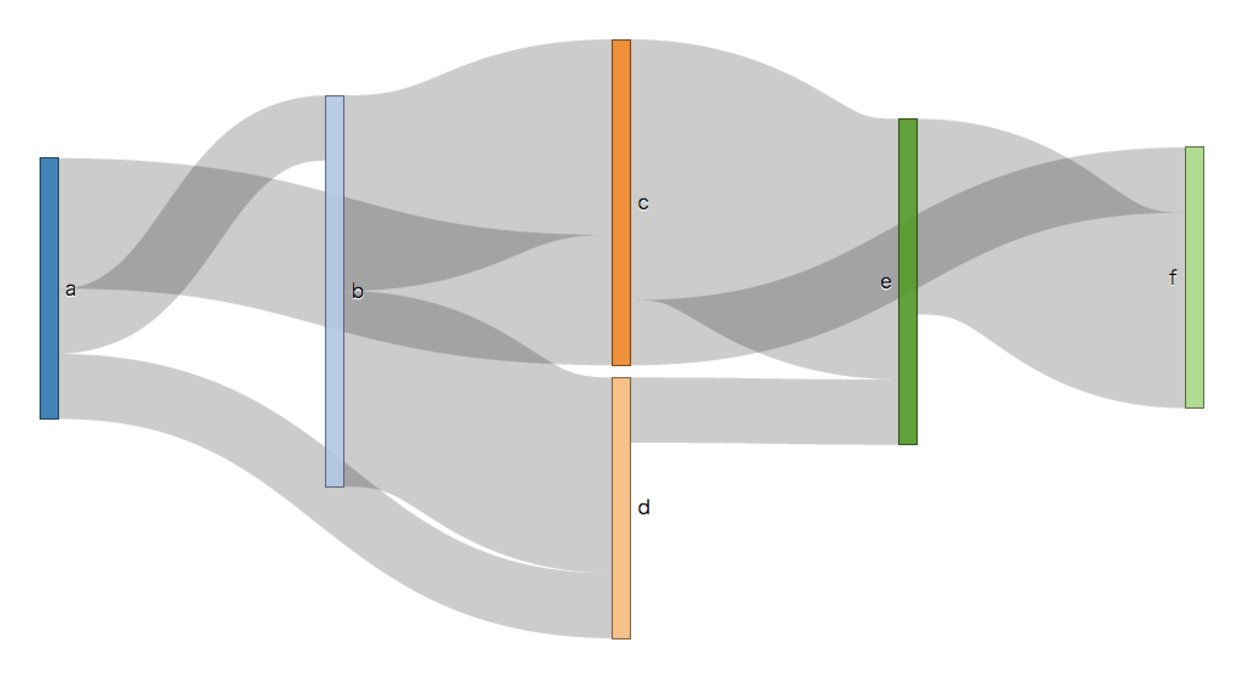
\includegraphics[scale=0.5]{figure/sankey1.eps}
\caption{sankeyダイアグラム\label{fig:sankey1}}
\end{center}
\end{minipage}

\end{tabular}
\end{center}
\end{figure}



\subsection{書式}
\begin{verbatim}
msankey [i=] f= v= [o=] [t=] [T=] [h=] [w=] [-nl] [--help] 
\end{verbatim}

\begin{table}[htbp]
{\small
\begin{tabular}{ll}
\verb|i=| & : 枝データファイル \\
\verb|f=| & : 枝データ上の2つの節点項目名 \\
\verb|v=| & : 枝の重み項目名 \\
\verb|o=| & : 出力ファイル(HTMLファイル) \\
\verb|t=| & : タイトル文字列 \\
\verb|-T| & : ワークディレクトリ(default:/tmp) \\
\verb|h=| & : キャンバスの高さを指定 \\
\verb|w=| & : キャンバスの幅を指定 \\
\verb|-nl| & : 節点項目名なし \\
\verb|--help| & : ヘルプの表示 \\
\end{tabular} 
}
\end{table} 

\subsection{利用例}
\subsubsection*{例1: 基本例}

前節の解説で用いてる例。


\begin{Verbatim}[baselinestretch=0.7,frame=single]
$ more dat1.csv
node1,node2,val
a,b,1
a,c,2
a,d,1
b,c,3
b,d,3
c,f,1
c,e,4
d,e,1
e,f,3
$ msankey.rb i=dat1.csv f=node1,node2 v=val o=output.html
$ head output.html
<!DOCTYPE html>
<html class="ocks-org do-not-copy">
<meta charset="utf-8">
<!--
<title>Sankey Diagram</title>
-->
<title></title>
<style>
\end{Verbatim}


%\end{document}
